\section{Experiment 2: Acceptance of the Robot Programming Framework}
\label{sec:Exp2}

In this experiment, we are addressing the following question:

\begin{enumerate}
  \item[\textbf{Q2}] Can users teach a robot action models for automated planning using the proposed framework iRoPro?
\end{enumerate}
\begin{sloppypar}
Users were presented a simulated implementation of iRoPro and had to teach action models by kinesthetic manipulating a Baxter robot (\fig{fig:Baxter}). 
Users were instructed to teach an atomic action by demonstration and assign preconditions and effects.
The goal was to assess the framework's usability and the user's difficulties encountered during the programming process.
At the end, participants were given a questionnaire related to their experience, their perceived understanding of the presented planning concepts and the usability of the framework.
In the following sections we briefly outline the experimental setup, measurements and results of the experiment.
The experimental protocol, questionnaire and additional material used can be found in Appendix \ref{app:exp2}.
%We then provide details on the partial implementation of the system used with the Wizard-of-Oz technique (\sect{ssec:WoZ}).
\end{sloppypar}

\subsection{Experimental Setup \& Participants}
We recruited 11 participants (7 male, 4 female), who were students and staff members at the Universit\'{e} Grenoble Alpes. 
6 participants reported programming experience with office productivity software (`beginner'), 2 had previously taken a programming course before (`advanced'), and 3 were pursuing studies in Computer Science (`expert').
%4 participants had previously heard of Automated Planning, but only 3 attended a related course.
The experiments were conducted using a Baxter robot (\fig{fig:Baxter}), mounted with a partial implementation of the framework.
The implemented functionalities included:
\begin{itemize}
	\item `learn new action': record the action demonstration
	\item `find a coloured object': apply the recorded action to an object of the specified colour
	\item `execute an action sequence': execute multiple actions
\end{itemize}

We used the Wizard-of-Oz technique to simulate the remaining functionalities (\eg `learn action preconditions and effects', `generate solution using a planner').
%Further details to the partial implementation are discussed in Section \ref{ssec:WoZ}.
Participants operated on a table with 2 positions D (for departure) and A (for arrival), 2 cubes (blue and red), that represented parts on an assembly line (\fig{fig:Baxter}). 
Each participant was allocated 1 hour, but the average duration was 29.5 minutes. 
The experiments were recorded, while the participant interacted with the robot. 


%The complete experimental protocol is shown in \fig{fig:Experimental protocol}. 
\subsection{Experimental Design \& Measurements}
The experiment scenario was set in a simulated assembly line, where objects of the same shape, but different colour arrived consecutively at the departure position D.
Users were told that objects were too heavy for human operators to move, hence needed to be handled by robots.
Also, due to the type of object, they should not be stacked.
Users had to teach Baxter the action for moving an object from D to arrival position A, for another maintenance task to be performed.
Throughout the experiment, users were faced with two different scenarios, where Baxter had to apply the learned move action. 
We evaluated the user's capability to refine action models and their associated conditions, when faced with different situations, and wanted to assess the framework's overall usability.

\begin{figure}[h]
	\centering
	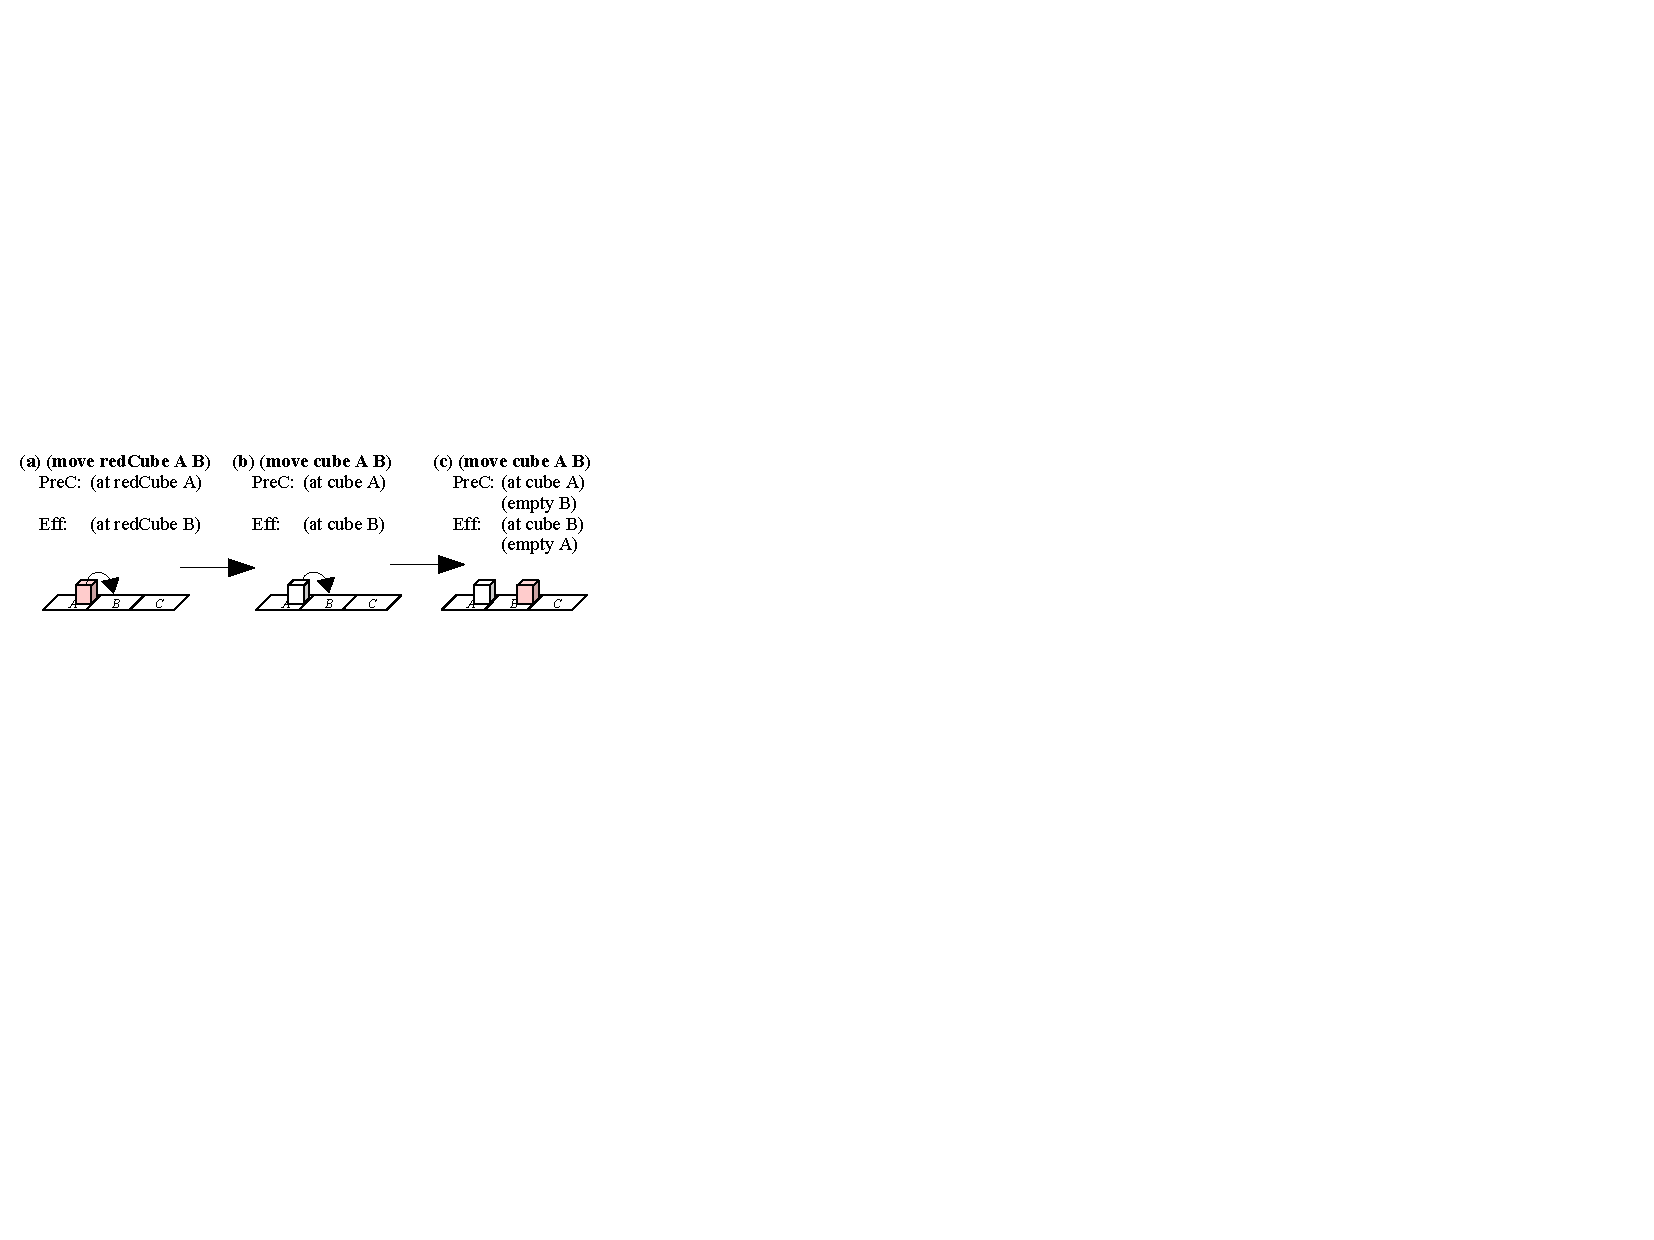
\includegraphics[width=0.8\linewidth]{figures/scenarios-exp2}
	\caption{Continuous refinement of the move action model: (a) initial action model learned by demonstration, (b) action model for all cubes of any colour, (c) action model with an additional condition, if the target position is occupied and cubes can not be stacked.}
	\label{fig:scenarios-exp2}
\end{figure} 

The experiment consisted of the following phases:
\begin{itemize}
  %\item{Introduction: After a short introduction to the Baxter robot \cite{Baxter}, users were told that they needed to use a planning language (STRIPS) to explain Baxter the state of the world and the semantic meaning of the actions.}
  \item{\textbf{Training:} Users were shown how to manipulate Baxter's arm, and given time to familiarise themselves with the kinesthetic manipulation. 
  	For this experiment we only used the robot's suction gripper to manipulate objects.}
  \item{\textbf{Experimental test:} Users were instructed to teach Baxter a move action of a red cube. 
  	Then, they were presented the action model, with preconditions and effects, that Baxter learned from the demonstration (\fig{fig:scenarios-exp2}a). 
  	In the following, users were faced with two different scenarios to refine the conditions of the action model. 
  	Starting with the initial action model for a red cube, users modified the conditions, so that it was applicable to all cubes of any colour (\fig{fig:scenarios-exp2}b), and when the target position was occupied (\fig{fig:scenarios-exp2}c). 
  	At each step, users observed how Baxter executed the learned action in the new scenario. 
  	When Baxter failed to execute the action, users had to refine the conditions of the action model.}
  \item{\textbf{Planning:} Users were presented a new scenario, where Baxter was instructed to achieve a goal using the learned action model. 
  	The new goal was to switch the positions of two cubes on the table (\fig{fig:planning-permutation}). 
  	Users first asked if they believed Baxter was able to solve this task and then shown how the taught action was reused with a task planner.
  	Finally, Baxter executed the action sequence to complete the task.}
  \item{\textbf{Questionnaire:} Users were given a questionnaire containing 18 questions related to their experience (\eg `I did not encounter any difficulties during the experiment') and their perceived understanding of the presented concepts (\eg `I can explain how Baxter represented the preconditions of a new action'), and the usability of the framework (\eg `No programming experience is required to teach Baxter a new task').
  Participants had to give a rating on a scale ranging from `Strongly agree', `Somewhat agree', `Somewhat disagree', and `Strongly disagree'.
  The complete questionnaire can be found in Appendix \ref{app:exp2}.}
   \item{ \textbf{Debriefing:} Throughout the experiment, users were asked about their expectations on Baxter's behaviour before applying the learned action model to a new scenario. 
   	Users were asked open-ended questions (\eg ``What will Baxter do when applying the learned action model?"), so that their responses were unbiased. 
   	When they encountered failure scenarios (\eg when Baxter stacked two cubes), they were asked to reason about Baxter's behaviour and proposed modifications to the taught action model.} 
\end{itemize}

\subsection{Results}
During the experiments we observed how users learned and used the presented programming process and planning concepts.
When asked for improvements of the initial action model (\fig{fig:scenarios-exp2}a) no users pointed out missing conditions before being faced with the new scenario (\fig{fig:scenarios-exp2}c).
Even users who were `experts' and who have heard of automated planning before, did not propose a complete action model from the start. 
However, when faced with the relevant failure scenarios all of the users detected the missing conditions easily.
In the final phase, 8 (or 73\%) users with no experience in automated planning did not expect Baxter to solve the permutation problem, and agreed unanimously that it acted in an intelligent manner, when it did. 

Figure \ref{fig:eEvaluation} shows the user responses to the questionnaire.
All 11 users were satisfied with the PbD process and Baxter's abilities to learn and reproduce the demonstrated move action and no users encountered difficulties during the experiment. 
%All users understood the learned action model and managed to adopt the notions of preconditions and effects easily. 
At the end of the experiment, all of the users believed that they had taught Baxter a new task. 
The majority of of the users were confident that they could explain how Baxter learned and represented the new action model.
9 (or 82\%) understood the notion of preconditions and agreed that no programming experience was required to teach Baxter using the proposed framework.


\begin{figure}[h]
	\centering
	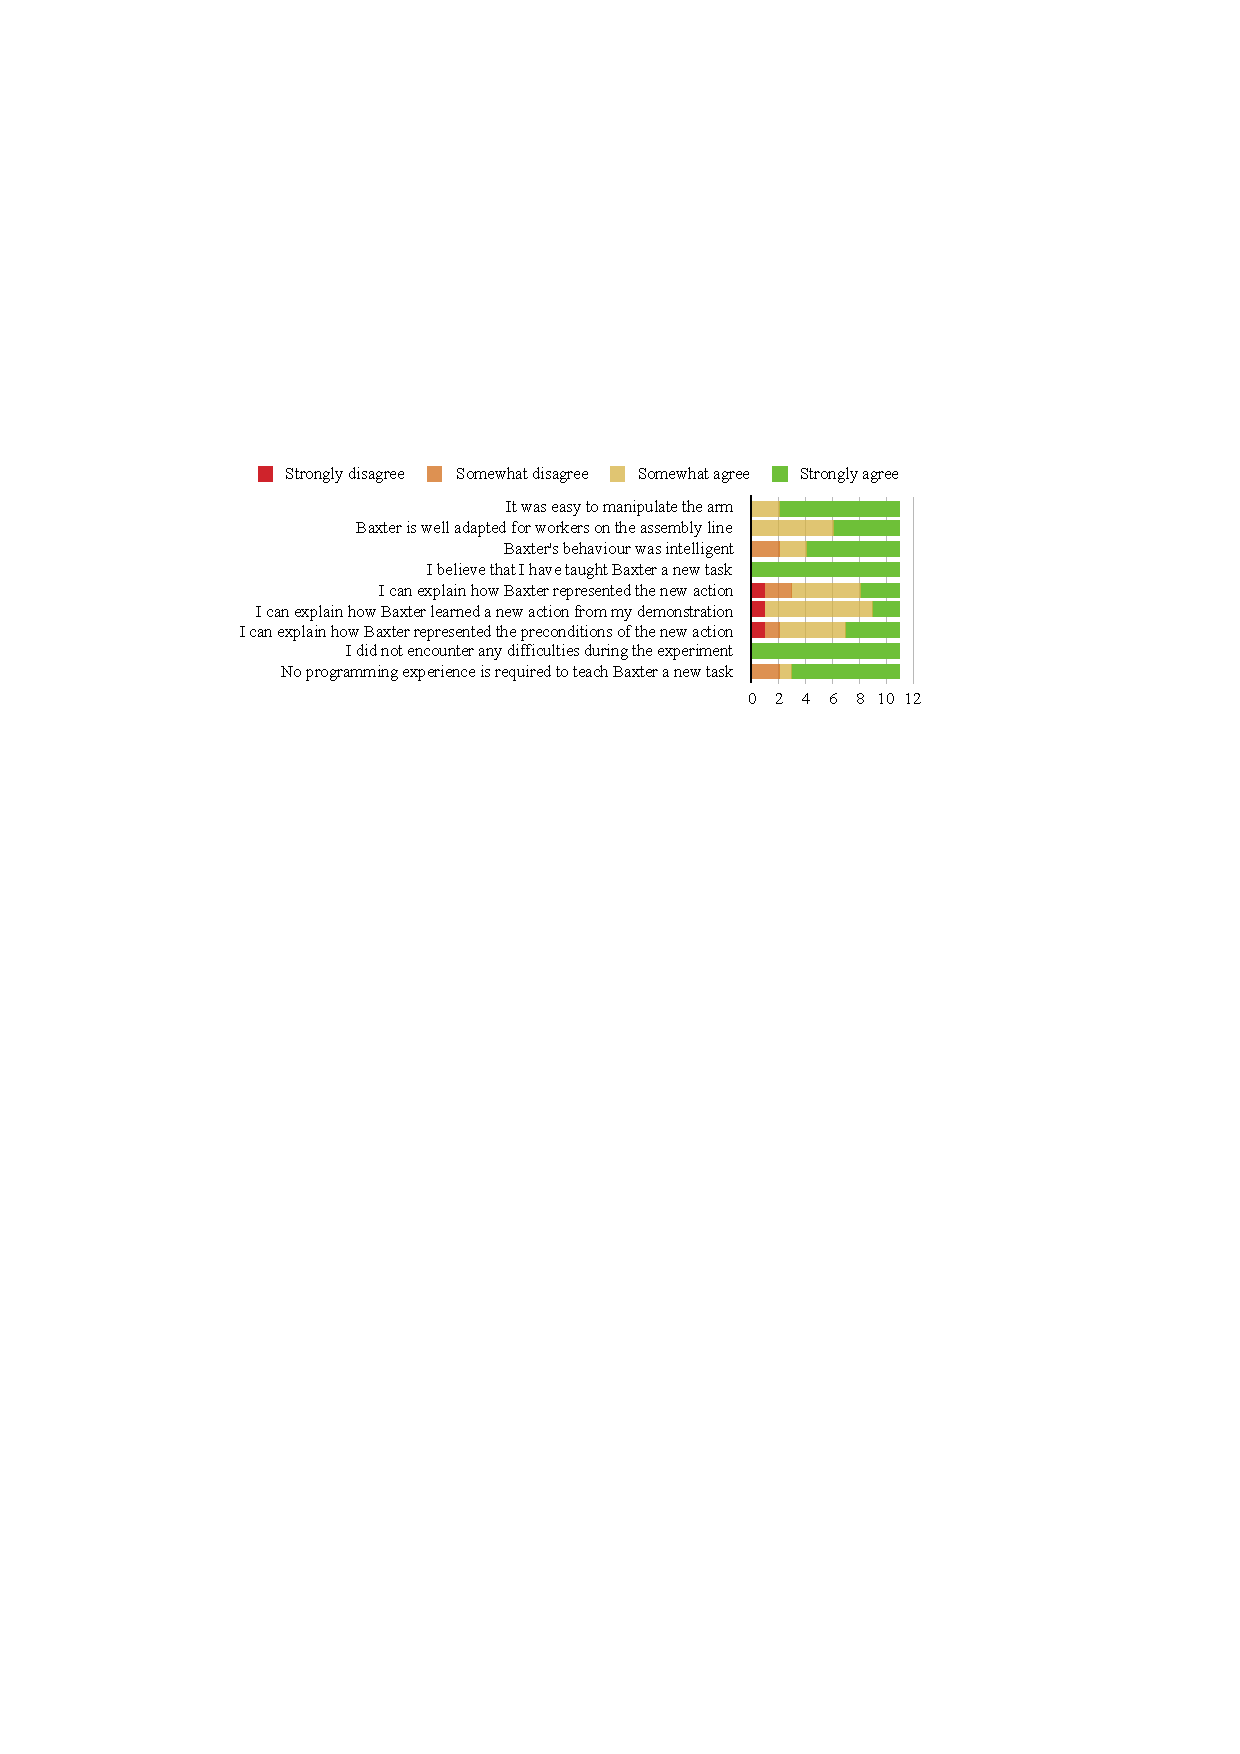
\includegraphics[width=\linewidth]{figures/eEvaluation}
	\caption{Summary of questionnaire responses: Extract of 18 questions on the user's perceived usability and understanding of the programming process after the experiment.}
	\label{fig:eEvaluation}
\end{figure}